\chapter{\IfLanguageName{dutch}{Stand van zaken}{State of the art}}
\label{ch:stand-van-zaken}

In het vorig hoofdstuk werd deze bachelorproef al kort ingeleid. In dit hoofdstuk zal de huidige kennis binnen dit onderzoeksdomein verder besproken worden.

In sectie \ref{sec:chatbots} zal er besproken worden wat chatbots zijn, welke soorten er bestaan, wat de voor -en nadelen zijn, wat de verbeterpunten en toekomstmogelijkheden zijn en hoe chatbots er nu voorstaan op het vlak van beveiliging en hoe dit verbeterd kan worden.

In sectie \ref{sec:nlp} wordt er ingezoomd op Natural Language Processing en de subdomeinen NLU en NLG.

In sectie \ref{sec:nlp-platformen} zullen de interessantste platformen kort geïntroduceerd worden en zullen ze vergeleken worden met elkaar op basis van een aantal basiscriteria. Binnen dit onderzoek worden geen volledig betalende NLP-platformen opgenomen.

\newpage
\section{Chatbots}
\label{sec:chatbots}

\subsection{Soorten}
\label{subsec:soorten}

\subsubsection{Rule-based chatbot}
\label{subsubsec:chatbots-soorten-rule-based-chatbot}

Dit is het eenvoudigste, maar het traagste type chatbot. Deze bot gebruikt geen machine learning of artificiële intelligentie, maar werkt op basis van voorgeprogrammeerde regels. Bij dit type kan je enkel communiceren via een vaste selectie vragen en bevelen. Bij antwoord van de chatbot, kun je ook enkel terug antwoorden uit een beperkt aantal mogelijke antwoorden uit een lijst. Dit type zorgt voor weinig vrijheid, waardoor het enkel inzetbaar is voor basis klantvragen. Doordat alles manueel geprogrammeerd moet worden, is het telkens veel werk om nieuwe regels toe te voegen en de functionaliteit uit te breiden. Indien je een bericht stuurt naar deze bot die hij niet kent, dan weet hij ook niet wat hij hiermee moet doen. Het grote voordeel van dit type is dat hij altijd accuraat antwoord geeft, net doordat alles voorgedefinieerd is. Binnen deze bachelorproef zullen chatbots van dit type niet verder onderzocht en toegelicht worden.

\begin{figure}[!htbp]
    \label{fig:rule-based-chatbot-example}
    \centering
    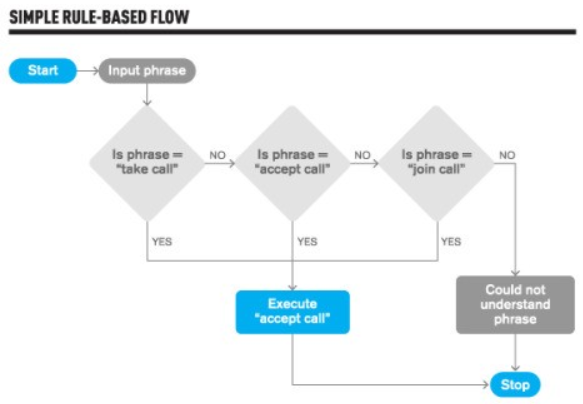
\includegraphics[width=0.8\textwidth]{rule-based-chatbot-example}
    \caption{Eenvoudige flowchart van een rule-based chatbot \autocite{Shridhar2017}}
\end{figure}

\subsubsection{ML-based chatbot}
\label{subsubsec:chatbots-soorten-ml-based-chatbot}


Dit type chatbot wordt ook wel de NLP-chatbot of de AI-powered chatbot genoemd. Bij deze soort wordt in tegenstelling tot de rule-based chatbot wel sterk gebruik gemaakt van artificiële intelligentie en machine learning. De bot kan vragen beantwoorden die hij nog nooit eerder heeft gekregen en elimineert dus de limitatie van het rule-based type. NLP-chatbots leren van voorgaande taken en maken zichzelf op deze manier slimmer en breiden hun kennis uit. Ze gebruiken ook speciale functies en algoritmes om de zinnen beter te verstaan en verder te verwerken. Dit type biedt de gebruiker veel meer vrijheid, maar is moeilijker om te ontwikkelen. De accuraatheid van deze soort is dan ook gemiddeld lager. Binnen deze bachelorproef zal de focus enkel liggen op chatbots van dit type. Wanneer er gesproken wordt over chatbots of gewoonweg bots, wordt er steeds een chatbot van dit type bedoeld.

\subsection{Voor- en nadelen}
\label{subsec:chatbots-voor-en-nadelen}

\subsubsection{Voordelen}
\label{subsubsec:chatbots-voor-en-nadelen-voordelen}

\begin{itemize}
    \item \textbf{Menselijke taken overnemen:} \\
    
    Chatbots worden ingezet voor heel wat verschillende toepassingen en kunnen menselijke taken overnemen. Een voorbeeld hiervan is het plannen van een meeting met een aantal personen. Het is vaak niet eenvoudig om een tijdstip te vinden die goed past in ieders agenda, daarom kan er bijvoorbeeld een chatbot worden gebruikt die dit voor ons kan doen op basis van een aantal namen die hij ontvangt die aanwezig moeten zijn. Chatbots nemen ook werk van de werknemers van klantendiensten en callcenters over, door de grote hoeveelheid mensen die er kunnen geholpen en bereikt worden op hetzelfde moment. Menselijke werknemers kunnen maar één persoon op hetzelfde moment verder helpen, bij chatbots is er geen limitatie op het aantal conversaties op hetzelfde moment. \\
    
    \item \textbf{Snellere interactie tussen onderneming en klant:} \\
    
    Uit een studie van \textcite{Social2016} blijkt dat klanten er van uit gaan dat er binnen de vier uur een antwoord wordt gegeven als er contact wordt opgenomen met de klantenservice via social media. Nu blijkt dat er in de realiteit een gemiddelde van tien uur tussen zit voordat er een antwoord wordt gegeven. Dit probleem wordt met chatbots opgelost, omdat er real-time communicatie is tussen klant en bedrijf. Er wordt direct een antwoord gegeven en dat heeft een positieve invloed op de tevredenheid van klanten en het succes van ondernemingen. \\
    
    \item \textbf{Herkenbare interface:} \\
    
    Mensen zijn tegenwoordig volledig thuis binnen de verschillende messaging apps (Facebook Messenger, WhatsApp, Slack, …), omdat veel mensen het dag in dag uit gebruiken om te communiceren met vrienden, familie en collega’s. Chatbots bieden een conversationele interface aan die heel erg gelijklopend is met de interface waarmee mensen comfortabel zijn. Soms zijn ze zelf volledig hetzelfde, bijvoorbeeld door een integratie met Facebook Messenger, WhatsApp of Slack. Doordat het vertrouwd overkomt, zullen mensen minder twijfelen om er gebruik van te maken. \\
    
    \item \textbf{Altijd beschikbaar:} \\
    
    Doordat chatbots geautomatiseerde gesprekspartners zijn, kunnen ze een hele dag doorwerken zonder onderbrekingen. Dit biedt voor gebruikers de mogelijkheid om eender wanneer op de dag gebruik te maken van deze systemen. \\
    
    \item \textbf{Kosten besparen:} \\
    
    Zonder een chatbot krijgt een bedrijf vaak dezelfde standaardvragen van klanten. Om al deze vragen te beantwoorden zijn werknemers nodig. Personeel moet natuurlijk betaald worden en werknemers kunnen menselijke fouten maken. Door het implementeren van een bot, is er een aanzienlijke hoeveelheid werk dat geautomatiseerd wordt en dus geen menselijke acties meer vereist. Op die manier kan een bedrijf op kosten besparen. \\
    
    \item \textbf{Data gebruiken voor verbeteringen:} \\
    
    Alle data die wordt verstuurd van en naar chatbots kan gemonitord en geanalyseerd worden. Daaruit kan er worden afgeleid hoe de organisatie nog beter kan inspelen op de specifieke noden en eisen van het doelpubliek. \\ 
    
\end{itemize}

\subsubsection{Nadelen}
\label{subsubsec:chatbots-voor-en-nadelen-nadelen}

\begin{itemize}
    \item \textbf{Extra mogelijkheden voor cybercriminelen:} \\
    
    Mensen sturen regelmatig gevoelige informatie naar chatbots zoals kredietkaartgegevens, betalingsinformatie en wachtwoorden. Dit biedt voor cybercriminelen nieuwe mogelijkheden om deze informatie te onderscheppen en te misbruiken. Het is belangrijk dat er hier de nodige aandacht aan besteed wordt voor de veiligheid van de consument. \\
    
    \item \textbf{Kan uit de hand lopen bij slechte supervisie:} \\
    
    Bots gaan zichzelf slimmer maken aan de hand van de informatie die ze toegestuurd krijgen. Dit betekent dat het belangrijk is dat wij, als mensen, goed monitoren wat er allemaal gebeurt, zodat niets uit de hand loopt. Een voorbeeld van slechte supervisie is de twitterbot Tay die in 2016 werd ontworpen door Microsoft als een experiment. Mensen stuurden deze chatbot racistische informatie door en na minder dan een dag stuurde de bot zelf racistische tweets de wereld in. Kort daarna werd het experiment stopgezet \autocite{Vincent2016}. \\
    
\end{itemize}

\subsection{Verbetermogelijkheden}
\label{subsec:verbetermogelijkheden}

Volgens \textcite{Hussain2019} zijn er nog veel verbeterpunten mogelijk op het vlak van chatbots. Zo zou er meer focus moeten liggen op het beter verstaan van taalkundige elementen door bijvoorbeeld emotionele-en sentimentanalyses uit te voeren. Chatbots zijn geen menselijke gesprekspartners en hebben daardoor dus ook geen empathie, maar empathie kan belangrijk zijn om een conversatie goed te laten verlopen. Tegenwoordig wordt hier sterk op ingezet, maar tot op het heden, staat dit nog niet op punt. Er zou ook een betere standaard moeten zijn om de kwaliteit van chatbots te testen.

Een eerder onderzoek heeft aangetoond dat mensen anders communiceren als ze weten dat ze met een machine converseren. Zo zouden mensen hun taal aanpassen als ze tegen een chatbot praten, zoals mensen ook doen als ze bijvoorbeeld tegen een kind bezig zijn \autocite{Hill2015}. Het is uiteindelijk de bedoeling dat mensen niet weten ofdat ze tegen een chatbot praten of niet. Op die manier zullen ze hun taal niet aanpassen en zal het meest optimale resultaat behaald worden. Indien mensen niet kunnen bepalen ofdat ze tegen een machine of tegen een mens praten, dan wordt er aan de Turingtest voldaan. Dit is een test die in 1936 werd opgesteld door Alan Turing en werd uitgediept in zijn paper in 1950 \autocite{Turing1950}.

Er zijn ook nog heel wat scenario’s waarbij chatbots geen gunstige antwoorden geven. Volgens \textcite{BRAIN2019} verstaan chatbots in 59\% van de gevallen regelmatig de berichten niet zoals gehoopt en worden in 29\% van de gevallen accenten of taalvariaties niet correct verstaan. Er is dus zeker nog progressie nodig om het maximale uit chatbots te halen.

\subsection{Toekomstperspectief}
\label{subsec:toekomstperspectief}

Chatbots hebben veel groeimarge en zullen in de toekomst nog een stevigere marktpositie innemen. Volgens \textcite{Andreoli2017} is er potentieel voor conversationele banking. We komen in een tijdperk waarbij chatbots en messaging applicaties zoals Facebook Messenger, WhatsApp, … enorme populariteit verkrijgen, zelfs meer dan sociale media. De banking industrie moet mee in dat tijdperk, omdat chatbots bidirectionele interactie ondersteunen in real-time voor klanten, perfect geschikt zijn voor mobiele toestellen en zeer goed geïntegreerd kunnen worden in de verschillende messaging apps. Door in te spelen op deze technologieën, zullen banken meer klanten kunnen bereiken dan voordien.

Verder zullen chatbots volgens \textcite{Patel2020} ook op kwalitatief vlak sterk groeien in de toekomst. Zo zullen er betere sentimentanalyses uitgevoerd worden om beter de emotie van klanten in te schatten en gepast te verwerken zodat chatbots meer aangepaste antwoorden kunnen geven. Chatbots zullen ook beter in staat moeten zijn om dialecten en accenten goed op te vangen. Verder zullen ze in de komende jaren ook meer en meer deel worden van ons dagelijkse leven.  

Chatbots zullen zich in de toekomst ook meer gedragen als mensen, waardoor het onderscheiden van bots en echte gesprekspartners moeilijker wordt. Tegenwoordig gedragen bots zich nog vaak oppervlakkig en hebben ze geen persoonlijkheid, waardoor ze onnatuurlijk overkomen. Facebook is op dit moment sterk aan het inzetten op het geven van een echte persoonlijkheid aan hun chatbots. Daardoor zullen hun chatbots zich gedragen als een echt persoon met specifieke karaktereigenschappen \autocite{Carey-Simos2018}.

\subsection{Security}
\label{subsec:security}

Chatbots beloven veel voordelen, maar er is ook enige bezorgdheid rond de veiligheid van deze systemen. Chatbots bieden voor cybercriminelen nieuwe manieren aan om data te onderscheppen van gebruikers. Veel data die circuleert tussen mens en bot zijn niet gevoelig, maar soms kunnen kredietkaartgegevens, logingegevens en dergelijke wel passeren. Deze data mag natuurlijk niet onderschept worden, want dat zou problemen kunnen veroorzaken. Organisaties maken zich zorgen over de veiligheid van chatbots, waar informatie opgeslagen wordt en hoe alles beveiligd wordt \autocite{Shanbhag2018}.


Volgens \textcite{Shanbhag2018} zijn er een aantal manieren om de veiligheid van chatbots te verbeteren:

\begin{itemize}
    \item \textbf{End-to-end encryptie:} \\
    
    Data die verstuurd wordt is volledig versleuteld, waardoor het niet leesbaar is voor criminelen die het eventueel zouden onderscheppen. Enkel de zender en de ontvanger kunnen de berichten lezen. \\
    
    \item \textbf{Two-factor authenticatie:} \\
    
    De identiteit van de chatbotgebruikers moet bevestigd worden door twee verschillende kanalen. Voorbeelden van deze kanalen zijn webpagina’s, sms’en, vingerafdruk, etc. Deze techniek wordt tegenwoordig vaak gebruikt in veel verschillende toepassingen. Een voorbeeld hiervan is dat je bij het aanmelden op Google eerst een code moet ingeven die je via sms hebt ontvangen. \\
    
    \item \textbf{Authenticatie timeouts:} \\
    
    Gebruikers worden automatisch uitgelogd als ze voor een bepaalde tijd inactief zijn. \\
    
    \item \textbf{Biometrische authenticatie:} \\
    
    De identiteit van gebruikers wordt bevestigd door een vingerafdruk of door gezichtsherkenning. \\
    
    \item \textbf{Self-destructing messages:} \\
    
    Gevoelige data die wordt verstuurd over het kanaal, wordt niet bijgehouden en kan dus niet onderschept worden. \\
\end{itemize}

Een aantal van deze technieken worden in de meeste chatbots automatisch toegepast.

\newpage
\section{Natural Language Processing (NLP)}
\label{sec:nlp}

\subsection{Natural Language Understanding (NLU)}
\label{subsec:nlp-nlu}

Natural Language Understanding is een onderdeel van NLP en is een techniek die verantwoordelijk is om machines de menselijke taal te leren verstaan en interpreteren aan de hand van algoritmes. NLU gebruikt veel technieken zoals sentiments-en-contextuele analyses en gaat ook de relatie tussen woorden in zinnen achterhalen. Ook slecht gevormde zinnen en woorden moeten verstaan worden. Het doel van NLU is om de intentie van de berichten te achterhalen. Daarbij is NLU ook verantwoordelijk om de juiste parameters/entities te extraheren uit zinnen. Intenties kunnen op veel verschillende manieren geformuleerd worden. Bijvoorbeeld, de zin “welk weer is het buiten”,  kun je op verschillende manieren formuleren, maar de intentie blijft hetzelfde, namelijk weten welk weer het is.


\subsection{Natural Language Generation (NLG)}
\label{subsec:nlp-nlg}


Natural Language Generation is een ander onderdeel van NLP en is een techniek waarbij structurele data (input) wordt omgezet in natural language (menselijke taal). Menselijke tekst of spraak wordt dus gegenereerd door machines. In deze bachelorproef zal er niet verder worden ingegaan op NLG, maar zal de focus liggen op het begrijpend vermogen van de chatbots (NLU).


\subsection{NLP vs NLU}
\label{subsec:nlp-nlp-vs-nlu}


De termen NLP en NLU worden vaak met elkaar verward en door elkaar gebruikt, NLU is een onderdeel van NLP. Bij het verstaan van menselijke tekst, zal NLP kijken naar wat er is gezegd, terwijl NLU zal kijken naar wat er is bedoeld. NLP kan tekst en spraak analyseren en technieken toepassen met de bedoeling om menselijke input (ongestructureerde data) om te zetten in structurele data, maar de bedoeling/intentie van berichten achterhalen, is een specifieke taak van NLU. 

\begin{figure}[!htbp]
    \label{fig:nlp-nlu-nlg}
    \centering
    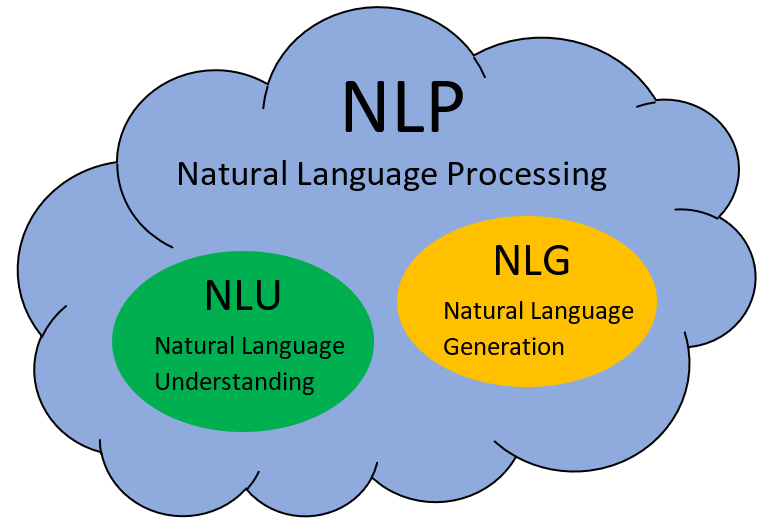
\includegraphics[width=0.5\textwidth]{nlp-nlu-nlg}
    \caption{Grafische voorstelling van NLP en de subdomeinen NLU en NLG}
\end{figure}

\section{NLP-platformen}
\label{sec:nlp-platformen}

Er zijn tientallen platformen op de markt waarmee chatbots gebouwd kunnen worden. De grootste en meest consistente platformen zijn ontwikkeld en onderhouden door de grote marktspelers zoals Google, Microsoft, IBM, Facebook en Amazon. Een chatbot is één van de vele dingen die gemaakt kan worden met deze platformen. Ze bieden een gebruiksvriendelijke interface aan, waarmee eenvoudig chatbots ontwikkeld kunnen worden. Ze hebben ook allemaal mogelijkheden voor hosting en ingebouwde integraties, waarmee de gebouwde applicaties zonder moeite op andere platformen gebruikt kunnen worden, zoals apps, websites, messaging apps, etc. Binnen vele studies worden de platformen van de grote marktspelers vaak naar voor geschoven in vergelijking met de kleinere. Daarom zal deze vergelijkende studie zich dan ook vooral focussen op platformen die door hen zijn aangeboden, omdat zij het kapitaal en de mogelijkheden hebben om te blijven innoveren en hun platformen verder te ontwikkelen. Er zal één platform worden onderzocht dat nogal sterk afwijkt van de andere, namelijk Rasa. Dat is omdat dit platform vaak sterk concurreert binnen vergelijkende studies met de andere traditionele. Er zullen enkel platformen worden bekeken die ondersteuning aanbieden voor de Nederlandse taal, omdat dit een absolute vereiste is voor klanten van In The Pocket die op de belgische markt actief zijn. Het platform van Amazon zal niet worden opgenomen, omdat hun tool geen Nederlands ondersteunt. Verder zullen er ook geen betaalde platformen worden opgenomen, want daar is er geen budget voor in deze bachelorproef.

\subsection{Dialogflow}
\label{subsec:nlp-platformen-dialogflow}

Dialogflow (vroeger API.ai) is een NLP-platform waarmee verschillende zaken ontwikkeld kunnen worden op basis van natuurlijke taal (Natural Language). Het platform is grotendeels gratis, maar de enterprise edities bieden nog uitgebreidere functies aan. Het is ontwikkeld en onderhouden door Google en maakt gebruik van de infrastructuur en ML-algoritmes van Google. Dialogflow is onderdeel van het Google Cloud Platform (GCP), dat is een platform die diensten aanbiedt voor applicatie infrastructuur, gegevensbeheer, analyses, machine learning en artificiële intelligentie, beveiliging, etc. Dialogflow is geoptimaliseerd voor het gebruik van Google Assistant. Er is ook ondersteuning voorzien voor meer dan twintig talen en er zijn veel intents en entities voorzien die je als ontwikkelaar zomaar kunt gebruiken. Er zijn al voorgebouwde chatbots aanwezig voor vaak voorkomende scenario’s die je kunt gebruiken. Dit platform kan ook geïntegreerd worden in andere diensten. Grote bedrijven zoals Domino’s Pizza, Mercedes, Comcast, Ticketmaster en Giorgio Armani maken onder andere gebruik van Dialogflow voor hun chatbots \autocite{Dialogflow2020}. 

\subsection{IBM Watson}
\label{subsec:nlp-platformen-ibm-watson}

IBM Watson is het NLP-platform van IBM en is, zoals Dialogflow, geschikt voor het bouwen van chatbots. Dit platform is een onderdeel van IBM Cloud, waardoor veel diensten van daar gebruikt kunnen worden. Watson kan voor een beperkt aantal conversaties gratis worden gebruikt. Het is gebouwd op neurale netwerken, waardoor het goed kan bijleren van vorige conversaties. Het ondersteunt dertien talen en voorziet ingebouwde entities. Er zijn verschillende ingebouwde integratiemogelijkheden voorzien. IBM Watson staat gekend als een platform die erg gebruiksvriendelijk is en waarmee in korte tijd een chatbot kan opgezet worden. Met klanten als The North Face en Chevrolet moeten ze niet onderdoen voor de concurrenten \autocite{IBM2020}.


\subsection{LUIS}
\label{subsec:nlp-platformen-luis} 

LUIS is de NLU-tool van Microsoft en is een vaste waarde op de markt. Met LUIS kan geen volledige chatbot worden gebouwd, omdat het enkel NLU-diensten aanbiedt en dus enkel dient voor intent classificatie en niet voor het antwoorden naar eindgebruikers toe.  Het kan daarentegen wel makkelijk geïntegreerd worden met het Microsoft Bot Framework, waarin wel de logica zit om complexe dialogen te voeren. LUIS is ook onderdeel van Microsoft Azure, waardoor het  goed kan samenwerken met deze cloudfuncties. LUIS maakt gebruik van een speciale active learning technologie waardoor het beter overweg zou kunnen met nieuwe trainingsdata. Er zijn dertien talen ondersteund en het bevat opnieuw veel ingebouwde intents en entities \autocite{LUIS2020}.

\subsection{Wit.ai}
\label{subsec:nlp-platformen-wit.ai}

Wit.ai is een open-source platform die ontwikkeld is door Facebook. Het is volledig gratis en ondersteunt 130 verschillende talen, wat erg veel is in vergelijking met de voorgaande platformen. Het is een platform die gebouwd is door en voor ontwikkelaars en doordat het open-source is, is elke interactie gedeeld met de volledige community. Doordat het platform ontwikkeld is door Facebook, heeft het wel een beperkt aantal integraties (enkel websites, apps en Facebook Messenger) \autocite{Wit2020}.

\subsection{Rasa}
\label{subsec:nlp-platformen-rasa}

Het laatste platform dat onderzocht werd, is één die sterk afwijkt van de anderen. Het is verschillend, omdat het niet wordt aangeboden door een groot bedrijf zoals Google, Facebook of Microsoft, maar ook omdat het volledig open-source is. Het is geen platform die, zoals de rest, bereikt kan worden via het internet met een user interface. Dit framework moet gedownload worden en dan kan er lokaal een chatbot worden gebouwd. Indien dit platform bereikbaar moet zijn vanop het internet, dan moet de ontwikkelaar daar zelf voor instaan. Het kan wel, mits wat configuratie, op Google Cloud, Microsoft Azure of Amazon Web Services (AWS) gezet worden. Deze tool vereist meer technische kennis van ontwikkelaars, maar biedt wel meer mogelijkheden om een chatbot te bouwen die aangepast is aan de noden van een project. Rasa bestaat uit Rasa NLU en Rasa Core.  Rasa NLU staat in voor het classificeren van de intents en het verstaan van berichten. Rasa Core is een module die gemaakt is om dialogen te voeren. Binnen dit onderzoek zal enkel Rasa NLU gebruikt worden. Doordat Rasa open-source is, kan er zelf worden gekozen welke componenten worden gebruikt voor het classificren van de intents. Dit zorgt ervoor dat het mogelijk is om in elke taal een chatbot met Rasa op te zetten. Er zijn ook heel wat componenten beschikbaar om gebruik te maken van voorgemaakte entities en intents. Rasa wijkt sterk af van de andere platformen, maar is zeker interessant om te onderzoeken, omdat het in voorgaande studies vaak sterk uit de hoek kwam en omdat het heel sterk op maat geïmplementeerd kan worden \autocite{RASA2020}.

\subsection{Vergelijking van platformen}
\label{subsec:nlp-platformen-vegelijking-platformen}

\begin{center}
    \newcolumntype{P}[1]{>{\hspace{0pt}}p{#1}}
    \begin{longtable}{| P{2.2cm} | p{2.2cm} |  p{2.2cm} | p{2.2cm} | p{2.2cm} | p{2.2cm} |}
        \hline
        \textbf{Naam}                                                  &  \textbf{Watson}                                                              & \textbf{LUIS}                           & \textbf{Rasa}                                         & \textbf{Wit.ai}                                 & \textbf{Dialogflow}                                    \\  \hline
        \textbf{Provider}                                              & IBM                                                                     & Microsoft                      & Rasa Technologies Inc.                       & Facebook                               & Google                                        \\  \hline
        \textbf{Subjectieve gebruiksvriendelijkheid}                               & Hoog                                                                    & Gemiddeld                      & Laag                                         & Gemiddeld                              & Hoog                                          \\  \hline
        \textbf{Prijs initieel gebruik}                                & Gratis                                                                  & Gratis                         & Gratis                                       & Gratis                                 & Gratis                                        \\  \hline
        \textbf{Limieten gratis gebruik}                               & 10 000 API calls, 25 intents en 25 entities per maand                    & 10 000 API calls per maand      & Onbeperkt                                    & Onbeperkt                              & 180 API calls per minuut                     \\  \hline
        \textbf{Ondersteunde talen}                                    & 13                                                                      & 13                             & 158                                     & 135                                    & 20                                            \\  \hline
        \textbf{Systeem intents}                                       & Nee                                                                     & Nee                & Ja, door specifieke componenten te gebruiken & Nee, Wit.ai bestaat enkel uit entities & Ja, uitgebreide lijst van voorgebouwde agents \\  \hline
        \textbf{Systeem entities}                                      & Ja, 5 in het Nederlands                                                 & Ja, 11 in het Nederlands       & Ja, door specifieke componenten te gebruiken & Ja, 26 in het Nederlands               & Ja, grote lijst voor het Nederlands           \\  \hline
        \textbf{Sentimentanalyse}                                      & Ja                                                                      & Ja                             & Ja                                           & Ja                                     & Ja                                            \\  \hline
        \textbf{Integraties met bestaande diensten}                    & 3 + alles van IBM Cloud                                                 & 11 + alles van Microsoft Azure & 9                                            & 1, Facebook Messenger                  & 18 + Alles van Google Cloud                   \\  \hline
        \textbf{Mogelijkheid tot integratie in eigen websites en apps} & Ja                                                                      & Ja                             & Ja                                           & Ja                                     & Ja                                            \\  \hline
        \textbf{SDK's}                                                 & C\#, Go, Java, Node.js, Python, Ruby, Android, Swift, Unity, Salesforce & C\#, Node.js, Python           & Python                                       & Node.js, Python, Ruby, Go              & C\#, Go, Java, Node.js, PHP, Python, Ruby     \\  \hline
        \textbf{Voorziet API om chatbot te gebruiken en beheren}       & Ja                                                                      & Ja                             & Ja                                           & Ja                                     & Ja                                            \\  \hline
        \textbf{Voorziet hosting}                                      & Ja                                                                      & Ja                             & Nee                                          & Ja                                     & Ja                                            \\  \hline
        \textbf{Spraakondersteuning}                                   & Ja                                                                      & Ja                             & Ja                                           & Ja                                     & Ja                                            \\  \hline
        \textbf{All-in-one platform}                                   & Ja                                                                      & Nee, enkel NLU                 & Ja                                           & Nee, enkel NLU                         & Ja                                            \\  \hline
        \textbf{Default fallback intent}                               & Ja                                                                      & Ja                             & Ja                                           & Nee                                    & Ja   \\ \hline    
        \caption{Vergelijkende tabel van de platformen op basis van de officiële documentatie waargenomen op 29 maart 2020}                                    
    \end{longtable}
\label{tbl:platformen}
\end{center}

In de bovenstaande tabel wordt gesproken over een default fallback intent, dat is een intent die aangeropen wordt als het model geen andere intent kan herkennen. Dit heeft als grote voordeel dat je een bericht naar de gebruiker kan sturen met het feit dat de chatbot het bericht niet goed heeft verstaan, wat de conversatie met de gebruiker actief houdt. Dit wordt verder niet meer besproken in deze bachelorproef, omdat dit niet relevant is voor dit onderzoek. De default fallback intent is wel opgenomen in de vergelijkende tabel, omdat dit een belangrijke functionaliteit kan zijn in de zoektocht naar het ideaal platform.

De platformen die hierboven besproken werden, werden ook al vaak in voorgaande studies met elkaar vergeleken. Uit deze studies bleken telkens andere platformen de bovenhand te nemen. Deze onderzoeken werden niet in het Nederlands gedaan, dus een Nederlandse vergelijking anno 2020 is dan ook zeker niet overbodig.

Volgens het onderzoek van \textcite{Russis2018} is de tool die IBM aanbiedt om chatbots in de cloud te bouwen veruit de beste op de markt met als dichtste achtervolgers Microsoft (LUIS) en Google (Dialogflow). Dit wordt dan weer betwist door het onderzoek van \textcite{Langen2017}, want zij besluiten dat LUIS (Microsoft) het betere platform is. De eerstvolgende achtervolger is Rasa, de resultaten van Rasa kwamen vrij dicht in de buurt van die van LUIS. Het groot voordeel van Rasa is dat het door de ontwikkelaar zelf geconfigureerd kan worden, waardoor het beter aangepast kan worden aan een specifieke use case. Rasa zou beter kunnen presteren dan LUIS als er meer configuratie op maat zou zijn. Dit maakt Rasa interessant om verder te onderzoeken. Volgens het onderzoek van \textcite{Savenkov2017} is ook IBM Watson de winnaar op het vlak van intent classificatie. Daarnaast zijn Api.ai (nu Dialogflow) en LUIS de eerstvolgende achtervolgers. De verschillen tussen die drie zijn relatief klein.

Een ander onderzoek geeft aan dat Snips.ai de beste oplossing voor intent classificatie is,  met als achtervolgers Wit.ai en Dialogflow \autocite{Coucke2017}. Snips.ai is een platform dat ook interessant is om verder te onderzoeken, maar dit platform ondersteunt geen Nederlands en is hierdoor niet relevant voor dit onderzoek.

Uit de verschillende onderzoeken hierboven beschreven kwamen vaak andere platformen naar boven met de beste prestaties voor intent classificatie. Er moet ook rekening gehouden worden met het feit dat deze onderzoeken al enige tijd geleden uitgevoerd zijn. De platformen en technologieën binnen AI en ML blijven ook continu evolueren, dit zorgt ervoor dat de resultaten nu volledig gewijzigd kunnen zijn. Deze bachelorproef zal hiervoor een oplossing bieden.

\begin{center}
    \begin{longtable}{| l | l | l | l | l | l |}
        \hline
        \textbf{Platform } &  \textbf{Watson} & \textbf{LUIS} & \textbf{Rasa}& \textbf{Wit.ai} & \textbf{Dialogflow} \\  \hline
        \textbf{\textcite{Russis2018}} & \cellcolor[rgb]{1,0.8431,0} \centering{1} & \cellcolor[rgb]{0.7529,0.7529,0.7529} 2 & & & \cellcolor[rgb]{0.80,0.50,0.20} 3 \\ \hline
        \textbf{\textcite{Langen2017}} & \cellcolor[rgb]{0.80,0.50,0.20} 3 & \cellcolor[rgb]{1,0.8431,0} 1 & \cellcolor[rgb]{0.7529,0.7529,0.7529} 2 & & \\ \hline
        \textbf{\textcite{Savenkov2017}} & \cellcolor[rgb]{1,0.8431,0} 1 & \cellcolor[rgb]{0.80,0.50,0.20} 3 & & & \cellcolor[rgb]{0.7529,0.7529,0.7529} 2 \\ \hline
        \textbf{\textcite{Coucke2017}} & & & & \cellcolor[rgb]{0.7529,0.7529,0.7529} 2 & \cellcolor[rgb]{0.80,0.50,0.20} 3 \\ \hline 
        \caption{Tabel die per onderzochte bron de platformen weergeeft die de het best scoorden op intentherkenning}                                    
    \end{longtable}
\end{center}














